\section{Design Process Models}

Design process models exist at the core of any engineering design exercise. They aid us in defining the approach and the key stages we will take to develop a solution to a given problem. Now, there are a large number of approaches that researchers and industry have developed over the years. \citeauthor{wynn2017}\cite{wynn2017} recent review of process models in design and development revealed that there are over 50 different models, which range from mapping the entire product development process to supporting specific elements of the process. These models also take different perspectives to how Engineering Design should be managed such as abstract, analytical, management science and procedural. 

\begin{figure*}[h!]
  \centering
  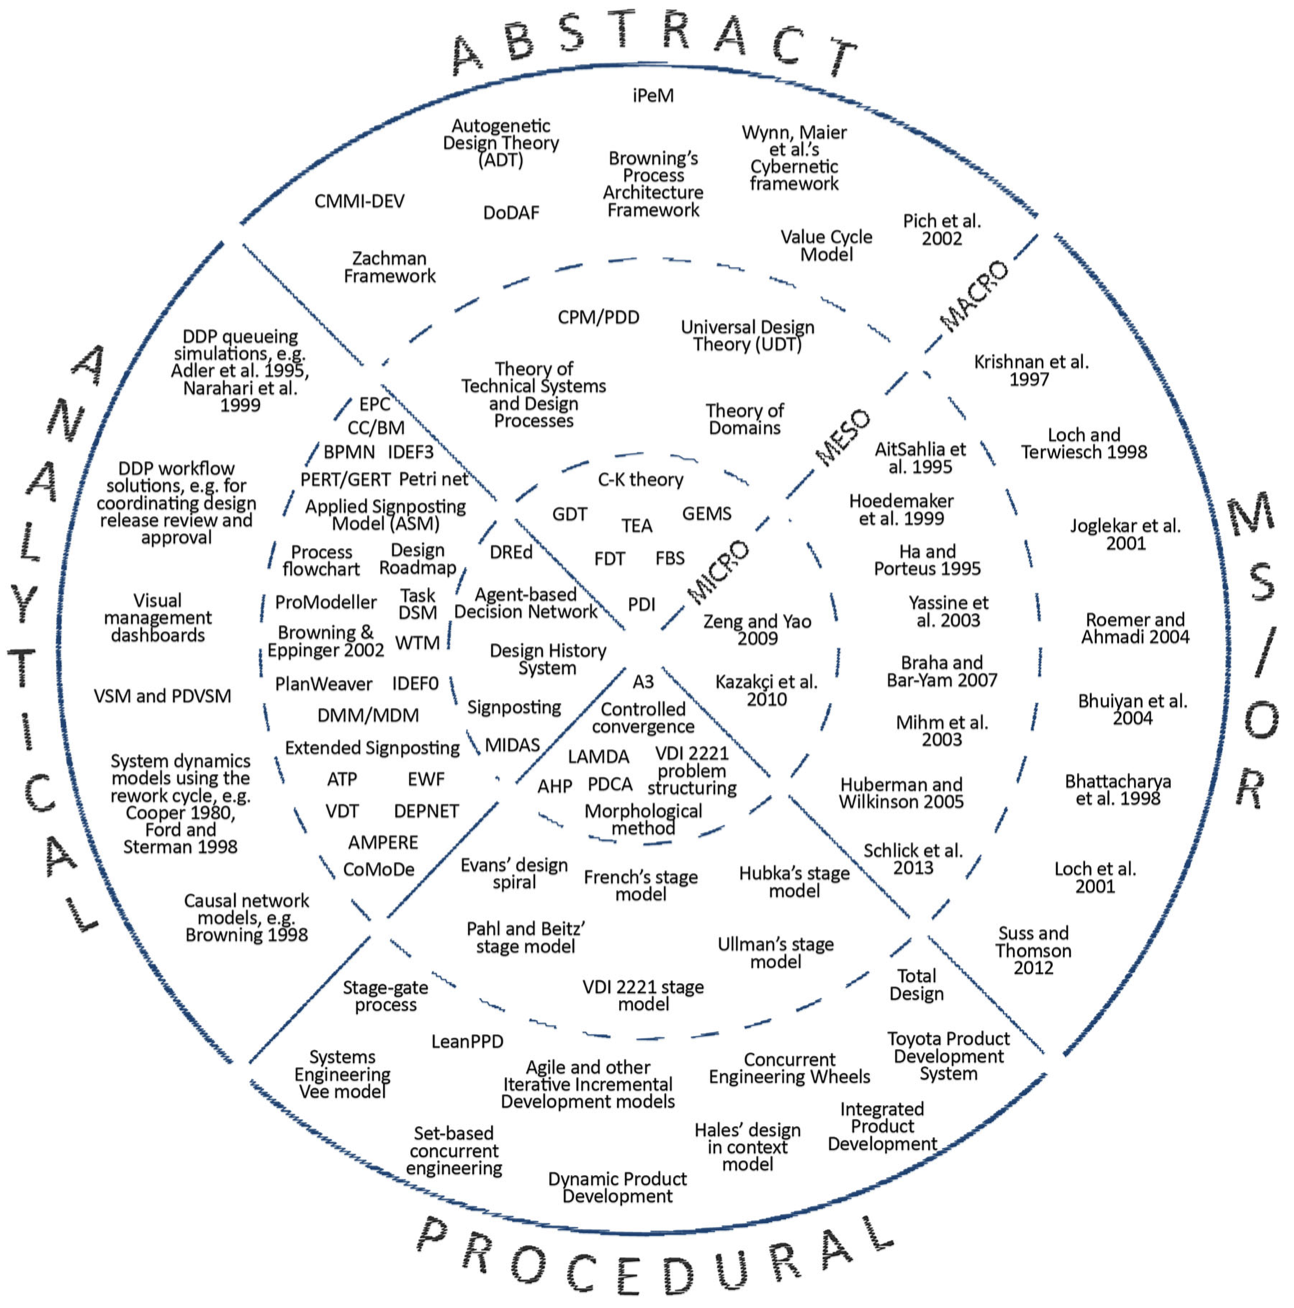
\includegraphics[width=0.8\textwidth]{03_design_process_models/wynn-review.png}
  \caption[Mapping of design process models against their scope and type]{Mapping of design process models against their scope and type~\citep{wynn2017}}
\end{figure*}


It is often the case that industry will customise a generic approach to fit their culture and domain. Many companies, particularly engineering consultancies, have identified that it is not only the solution but the process they take to solve problems that provides them with a competitive advantage in business. 

In this section, we will cover four commonly adopted models:

\begin{enumerate}
  %\item The Systematic Design Process VDI2221
  \item VDI2221 -- Systematic Design Process Model
  \item V-Model
  \item Design Double Diamond
  \item Stage-Gate Model
\end{enumerate}


\subsection{VDI2221 -- Systematic Design Process Model}

The \acf{VDI2221} was developed by senior designers from industry and academia. The aim was to provide a generic approach for the design of products within the fields of mechanical, precision, control, software and process engineering. The approach (\cref{fig-vdi}) includes seven basic working steps.

As this process was designed for general applicability, the \ac{VDI2221} has a very abstract structure, thus permitting product-specific and company-specific variations. \cref{fig-vdi} should therefore be regarded as a guideline to which detailed working procedures can be assigned. Special emphasis is placed on the iterative nature of the approach and the sequence of the steps must not be considered rigid. Some steps might be omitted, and others repeated frequently. This flexibility is in accordance with practical design experience and enables companies to frame their processes in a similar manner to enable communication of where they are in their product development cycle.

\begin{figure*}[h!]
    \centering
    \includestandalone[width=0.6\textwidth, mode=buildnew]{03_design_process_models/VDI2221}
    \caption[Systematic Design Approach]{Systematic Design Approach~\citep{pahl2013}}\label{fig-vdi}
\end{figure*}



\subsection{Design Double Diamond}

The Design Council\cite{council2007} illustrates the design process as a Double Diamond (\cref{fig-dd}), which is divided into four distinct phases:

\begin{enumerate}
    \item Discover
    \item Define
    \item Develop
    \item Deliver
\end{enumerate}

\begin{figure}[h!]
    \centering
    \includestandalone[width=0.7\textwidth, mode=buildnew]{03_design_process_models/double_diamond}
    \caption[Design Double Diamond]{Design Double Diamond}\label{fig-dd}
\end{figure}

In all creative processes a number of possible ideas are created (`divergent thinking') before refining and narrowing down to the best idea (`convergent thinking'), and this can be represented by a diamond shape. The Double Diamond indicates that this happens twice – once to confirm the problem definition and once to create the solution. One of the greatest mistakes is to omit the left-hand diamond and end up solving the wrong problem.

In order to discover which ideas are best, the creative process is iterative. This means that ideas are developed, tested and refined a number of times, with weak ideas dropped in the process. This cycle is an essential part of good design.

Practical design methods -- like user diaries, journey mapping and character profiles -- move a project through the four phases of the Double Diamond. 

The\marginnote{discover} first quarter of the Double Diamond model covers the start of the project. Designers try to look at the world in a fresh way, notice new things and gather insights.

The\marginnote{define} second quarter represents the definition stage, in which designers try to make sense of all the possibilities identified in the Discover phase. Which matters most? Which should we act on first? What is feasible? The goal here is to develop a clear creative brief that frames the fundamental design challenge.

The\marginnote{develop} third quarter marks a period of development where solutions or concepts are created, prototyped, tested and iterated. This process of trial and error helps designers to improve and refine their ideas.

The\marginnote{delivery} fourth and final quarter of the double diamond model is the delivery stage, where the resulting project (a product, service or environment, for example) is finalised, produced and launched.

\subsection{V-Model}

The V-Model \pref{fig-v-model} has been widely adopted across systems design where a product can be split into separate sub-systems that can be developed and tested independently from one another.
The left-hand side of the ``V'' details the processes that organisations follow to decompose the list of requirements for a product into a set of separate system element specifications that are then used to generate a set of designs for the sub-systems of the product.

The sub-systems can then be tested independently before being integrated until the full product is formed (right-hand side of the `V'). 
Testing is performed at each stage of the integration of the systems, which simplifies the identification of issues as the product is built-up.

\begin{figure*}[h!]
    \centering
    \includestandalone[width=0.8\textwidth]{03_design_process_models/v-model.tex}
    \caption{Systems Engineering V-Model}\label{fig-v-model}
\end{figure*}


\subsection{Stage/Phase-Gate Model}

Stage/Phase-Gate models arose during the management of large-scale projects for mechanical and chemical engineering in the 1940s. One of the major organisations to develop this model further was in the \acf{NASA}.
\ac{NASA} introduced its phased review process in the 1960s and broke up the development of their projects into a series of phases that could be individually reviewed.

\begin{figure*}
    \centering
    \includestandalone[width=0.9\textwidth]{03_design_process_models/stage-gate}
    \caption{Stage-Gate Model}\label{fig-stage}
\end{figure*}

The phased review process consisted of five stage with periodic development reviews between stages \pref{fig-stage}. 
The stages phases are:

\begin{table}
    \begin{tabular}{r l}
        Start & Discovery \& Idea Generation \\
        Stage 1 & Scoping \\
        Stage 2 & Building the Business Case \\
        Stage 3 & Development \\
        Stage 4 & Testing \& Validation \\
        Stage 5 & Launch \\
    \end{tabular}
\end{table}

The\marginnote{start} design team will be given a design brief that provides a high-level abstraction of a problem that they are trying to solve. From this, the organisation will begin to develop potential ideas that will solve this problem using concept generation techniques. 

These ideas will then be presented at the first gate review where they will follow a concept selection technique to decide which idea(s) will continue into the scoping stage of the project. It is not uncommon for more than one idea to continue into the next stage if budget and resource is available.

With\marginnote{stage one: scoping} the ideas selected, the project continues into Stage 1 of the model. This is where engineers evaluate the product and the market that it will be entering. Engineers need to consider the strengths and weaknesses of the product and what it is going to offer to the potential consumer. 

Analysis of the competition enables the organisation to estimate the level of market penetration the potential product might have. This information is then fed back into the review gate where the senior management team will decide whether to continue with the development of the product. Remember, this model is typically applied to large engineering projects that are potentially worth Millions or Billions of pounds. Thus, these organisations need to be clear of the business opportunity before committing their resources to a project.

If\marginnote{stage two: building the business case} a clear market gap and engineering solution has been presented, and the organisation has decided to go ahead, the engineers then move into Stage 2, which is to fully define and build the business case around the project. This is the last stage before the commitment of engineering work and resource is made to the project. Business cases and their format can vary considerably between industries but in general, they will include reports detailing the product definition, business case, project plan, and review of the projects' feasibility.

After\marginnote{stage three: development} review of the business case, the organisation will decide whether to continue on with the project. If accepted, the project moves into Stage 3, which is where the project is actually executed. This covers the product's design and development, and will include some early prototyping and stakeholder feedback.

The results of this stage is a fully-functional prototype of the product that is to be manufactured and sold. This will be taken into the review where it will be critiqued in relation to the PDS and further checking of the business case to ensure the opportunity in the market still exists.

With\marginnote{stage four: testing and validation} the prototype fully developed, the project can move into the testing and validation stage. This is where the prototype will be tested in a variety of use cases and provided to the stakeholders for trialling and feedback.

If\marginnote{stage five: launch} the testing and validation is successful, the organisation is now is ready to launch the product and ramp-up production.

\subsection{This Design Exercise}

In this exercise, we will be adapting \ac{VDI2221} and follow the process shown in \cref{fig-dm-process}.
The process has been developed to map with University timetabling and study hours for the course.

\begin{figure}[h!]
    \centering
    \includestandalone[width=0.65\textwidth]{03_design_process_models/design_and_make}
    \caption{Design \& Make Design Process}\label{fig-dm-process}
\end{figure}

The\marginnote{design brief} exercise will begin with a design brief and is the general problem that you're going to try and solve. In doing so, you will need to clarify elements of the task and start to build the boundaries and constraints in order to solve the design problem.

The\marginnote{product design specification} formalisation of these boundaries and constraints comes in the development of a \acf{PDS}. Your design will need to meet these requirements in order to be a valid solution to the problem. The PDS will be a mixture of subjective and objective requirements, which will be used to assess the viability of your design ideas. 

With\marginnote{concept generation} the requirements set, we will then move into the concept generation stage. This is where you will develop a number of concepts that will aim to meet the PDS. To develop these concepts, we will be discussing and applying some concept generation techniques. The aim of concept generation is to diverge by exploring the design space and developing as many potential ideas as possible. No matter how crazy they may seem!

Now\marginnote{concept selection} we have a number of potential concepts, we need to begin to converge by assessing the concepts against the \ac{PDS}. We will be introducing you to four techniques to do this.

\marginnote{embodiment design} Having selected the final concept, it is time to develop the concept further by refining how the components will interact and fix against one another. This is where engineers perform a comprehensive analysis of all the forces, heat transfer, fluid flow, system dynamics and/or kinematics relating to the product.

This provides us with a preliminary layout of all the components within the product and estimates for the component sizes.

This\marginnote{detail design} takes us into the detail design section of the design process and is where you will be selecting components, drawing up components for manufacture and developing the instructions for the assembly of the prototype. In this stage, you will be using the ideas from Design for Assembly and Design for Manufacture to further refine the design. The result will be the instructions of producing the parts, generating the purchase orders for the suppliers and creating a \acf{BOM} for the prototype.